Pierwszym krokiem algorytmu wykrywania logo \bk, jest przetwarzanie wstępne. Celem przetwarzania wstępnego jest zmniejszenie rzeczywistego rozmiaru obrazu, względna poprawa jego jakości oraz usunięcie zakłóceń.

\subsection{Skalowanie obrazu}
Celem skalowania obrazu jest stworzenie nowego obrazu o~zmienionym rozmiarze, wykorzystując do tego obraz oryginalny. W~przypadku projektowanego systemu, obraz analizowany jest poddawany skalowaniu aby zmniejszyć jego rzeczywisty rozmiar, celem uproszczenia dalszych obliczeń.

Do zmiany rozdzielczości obrazu cyfrowego zwykle wykorzystuje się metody interpolacji. Algorytmy tego typu można podzielić na algorytmy nieadaptacyjne oraz adaptacyjne. Pierwsza grupa dokonuje interpolacji w~ustalony z~góry sposób, niezależnie od zawartości przetwarzanego obrazu. Algorytmy adaptacyjne zmieniają sposób przetwarzania pikseli, biorąc pod uwagę cechy aktualnie przetwarzanego fragmentu. Adaptacja pozwala na zwiększenie jakości wizualnej, zwiększając przy tym koszt obliczeniowy~\cite{swierczynski2008podwyzszanie}.

W~ramach projektu przeanalizowałem działanie trzech algorytmów nieadaptacyjnych: 
\begin{itemize}
    \item interpolacja najbliższym sąsiadem,
    \item interpolacja dwuliniowa,
    \item interpolacja dwukubiczna.
\end{itemize}

Wymienione algorytmy różnią się ilością punktów branych pod uwagę podczas obliczania jasności piksela w~obrazie wynikowym. W~pierwszym kroku każdego algorytmu oblicza się w~którym miejscu w~obrazie wejściowym znajduje się rozpatrywany punkt obrazu wyjściowego. Dokonuje się tego poprzez obliczenie współczynników skalowania, zgodnie z~wzorami~\ref{eqn:wsp-skalowania-x}~i~\ref{eqn:wsp-skalowania-y}.

\begin{equation}
    \label{eqn:wsp-skalowania-x}
    r_{x} = \frac{\mathrm{width}_{input}}{\mathrm{width}_{output}}
\end{equation}

\begin{equation}
    \label{eqn:wsp-skalowania-y}
    r_{y} = \frac{\mathrm{height}_{input}}{\mathrm{height}_{output}}
\end{equation}

Na podstawie współczynników $r_{x}, r_{y}$ dla piksela $(i, j)$ obrazu wyjściowego oblicza się pozycję~$(x, y)$ w~obrazie wejściowym, wykorzystując zależność \ref{eqn:skalowanie}.

\begin{equation}
    \label{eqn:skalowanie}
    \begin{array}{ll}
        x = i \cdot r_{x} & y = j \cdot r_{y}
    \end{array} 
\end{equation}

\subsubsection{Interpolacja najbliższym sąsiadem}
Interpolacja metodą najbliższego sąsiada jest najprostszą metodą zmiany rozmiaru obrazu cyfrowego. Jest to metoda wymagająca najmniejszej mocy obliczeniowej i~jest jedyną metodą nie powodującą rozmycia obrazu wynikowego. W~przetwarzaniu obrazów jest najczęściej wykorzystywana do zmiany rozmiaru zdjęć zawierających kody kreskowe lub zrzutów ekranu aplikacji okienkowych.

Algorytm interpolacji najbliższym sąsiadem działa w~sposób przedstawiony na rysunku~\ref{fig:nn-example}. Dla każdej obliczonej pary $(x,y)$ odpowiadającej pikselowi $(i, j)$ w~obrazie wyjściowym, wybierany jest rzeczywisty piksel $(\hat{x}, \hat{y})$ obrazu wejściowego, którego odległość punktu docelowego jest najmniejsza (czyli jest najbliższym sąsiadem obliczonego piksela).

\begin{figure}[h]
    \centering
    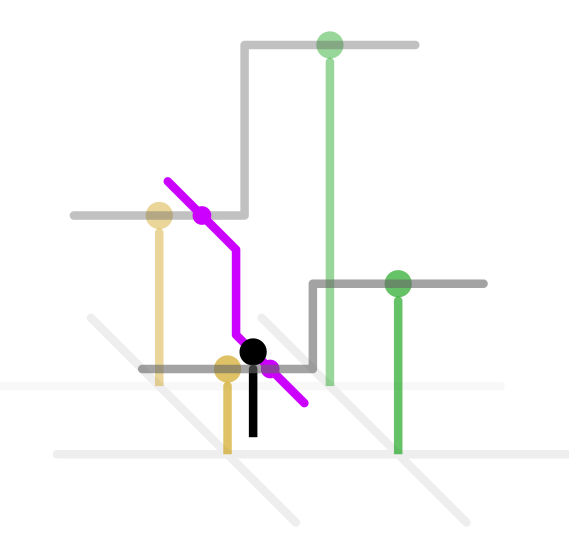
\includegraphics[width=0.6\columnwidth]{figures/nearestneighbour.png}
    \caption{Wybór najbliższego sąsiada w~algorytmie interpolacji~\cite{WikipediaEN:bicubicimg}}
    \label{fig:nn-example}
\end{figure}

W~stworzonym rozwiązaniu, algorytm interpolacji dwuliniowej jest implementowany przez  obiekty klasy \texttt{POBR::NearestNeighbourInterpolationResizer}. Wyniki działania tego algorytmu zostały przedstawione na rysunku~\ref{fig:nearestneighbour-result}. 

\begin{figure}[h]
    \centering
    \subfloat[25x25px]{{
\includegraphics[scale=2.6]{figures/25x25/nn.png}}}
    \qquad
    \subfloat[50x50px]{{
\includegraphics[scale=1.3]{./figures/50x50.jpg} }}%
    \qquad
    \subfloat[100x100px]{{
\includegraphics[scale=0.65]{./figures/100x100/nn.png} }}
    \caption{Efekt działania algorytmu interpolacji najbliższym sąsiadem na przykładzie zmniejszania logo \bk z~rozmiaru 50x50px do 25x25px oraz zwiększania do rozmiaru 100x100px}
    \label{fig:nearestneighbour-result}
\end{figure}

Obrazy przetworzone za pomocą algorytmu interpolacją najbliższego sąsiada cechują się blokowatością. Brak rozmycia powoduje że obraz traci naturalny wygląd. Jest to jednak metoda najszybsza, warta rozważenia w~zadanich automatycznego wykrywania obiektów.

\subsubsection{Interpolacja dwuliniowa}
Algorytm interpolacji dwuliniowej jest algorytmem nieadaptacyjnym, nieco bardziej zaawansowanym niż pokrewny algorytm najbliższego sąsiada. Wartość każdego piksela obrazu wynikowego jest obliczana na podstawie czterech sąsiednich punktów obrazu wejściowego~\cite{algorytmy:bilinear}.

Na podstawie informacji o~docelowym punkcie, wybiera się cztery najbliższe punkty $F_{0,0}, F_{0,1}, F_{1,0}, F_{1,1}$, tak jak to przedstawiono na~\ref{fig:bilinear-result} (żółtym kolorem zaznaczono punkt obliczony z~wzorów~\ref{eqn:skalowanie}). 

\begin{figure}[h]
    \centering
    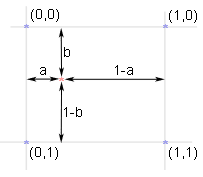
\includegraphics[width=0.6\columnwidth]{figures/bi2.png}
    \caption{Dobór sąsiednich punktów w~algorytmie interpolacji dwuliniowej~\cite{algorytmy:bilinear}}
    \label{fig:bilinear-example}
\end{figure}

Następnie trzykrotnie przeprowadza się interpolację pomiędzy punktami, najpierw dwa razy w~kierunku poziomym pomiędzy $F_{0,0}$~i~$F_{1,0}$ oraz $F_{0,1}$~i~$F_{1,1}$ i~ostatni raz pomiędzy wynikami poprzednich interpolacji, zgodnie ze wzorem~\ref{eqn:interpolacja}. Proces ten należy powtórzyć dla każdej składowej koloru z~osobna~\cite{algorytmy:bilinear}.

\begin{equation}
    \label{eqn:interpolacja}
    \begin{array}{l}
        F_{a,0} = (1-a) \cdot F_{0,0} + a \cdot F_{1,0} \\
        F_{a,1} = (1-a) \cdot F_{0,1} + a \cdot F_{1,1} \\
        F_{a,b} = (1-b) \cdot F_{a,0} + b \cdot F_{0,1} \\
    \end{array} 
\end{equation}

W~stworzonym rozwiązaniu, algorytm interpolacji dwuliniowej jest implementowany przez  obiekty klasy \texttt{POBR::BilinearInterpolationResizer}. Wyniki działania tego algorytmu zostały przedstawione na rysunku~\ref{fig:bilinear-result}.

\begin{figure}[h]
    \centering
    \subfloat[25x25px]{{
\includegraphics[scale=2.6]{figures/25x25/bl.png}}}
    \qquad
    \subfloat[50x50px]{{
\includegraphics[scale=1.3]{./figures/50x50.jpg} }}
    \qquad
    \subfloat[100x100px]{{
\includegraphics[scale=0.65]{./figures/100x100/bl.png} }}
    \caption{Efekt działania algorytmu interpolacji dwuliniowej na przykładzie zmniejszania logo \bk z~rozmiaru 50x50px do 25x25px oraz zwiększania do rozmiaru 100x100px}
    \label{fig:bilinear-result}
\end{figure}

Algorytm interpolacji dwuliniowej jest zdecydowanie bardziej skomplikowanym algorytmem przetwarzania. W~wyniku jego działania, obraz wyjściowy jest rozmyty, co jednak pozwala na zachowanie naturalnego wyglądu obrazu. Mimo brania pod uwagę czterech pikseli, metoda ta niewiele mocniej obciąża procesor. 

\subsubsection{Interpolacja dwukubiczna}
Interpolacja dwukubiczna jest najczęściej wykorzystywanym algorytmem zmiany rozmiaru obrazu, szczególnie w~system gdzie prędkość przetwarzania nie jest najważniejszym kryterium. Zamiast czterech najbliższych punktów, algorytm bierze pod uwagę szesnaście najbliższych punktowi docelowemu pikseli. Obrazy przetworzone przez algorytm dwukubiczny mają znacznie gładsze krawędzie oraz pozbawione są widocznych artefaktów.

\begin{figure}[h]
    \centering
    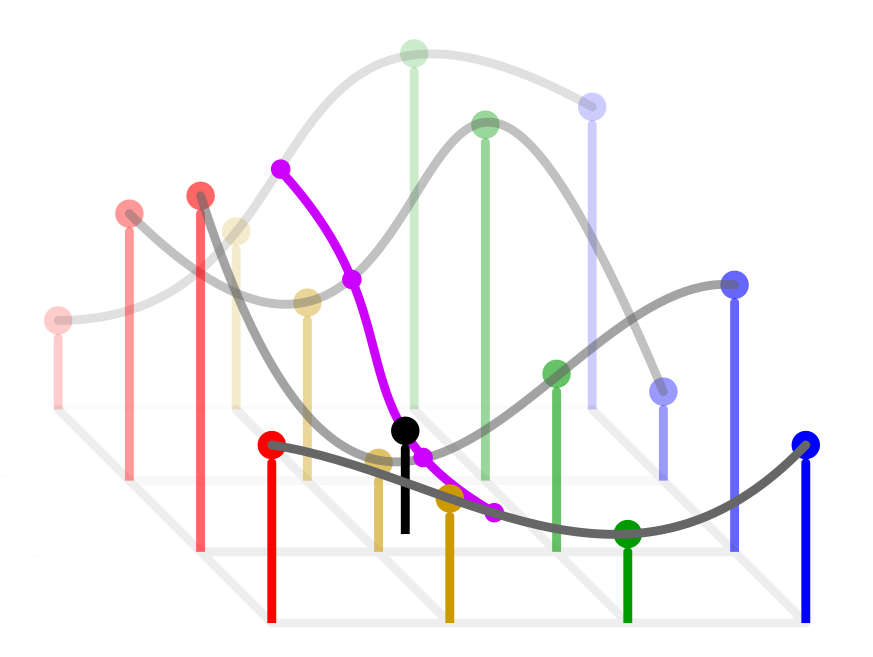
\includegraphics[width=\columnwidth]{figures/bicubic.png}
    \caption{Zasada działania algorytmu interpolacji dwukubicznej~\cite{WikipediaEN:bicubicimg}}
    \label{fig:bicubic-example}
\end{figure}

Poglądowo, zasada działania algorytmu została przedstawiona na rysunku~\ref{fig:bicubic-example}. Do wyznaczenia wartości jasności danego piksela, algorytm bierze pod uwagę szesnaście pikseli w~bezpośrednim otoczeniu wyznaczonej pozycji $(x,y)$ piksela. Podobnie jak w~alogrytmie dwuliniowym, w~pierwszej kolejności dokonywana jest interpolacja w~osi poziomej, tym razem jednak czterokrotnie, dla czterech rzędzów pikseli. Funkcje jasności są lokalnie interpolowane wielomianem trzeciego stopnia. Następnym krokiem algorytmu jest ponowna interpolacja, tym razem w~osi pionowej. Operację należy powtórzyć dla każdej zmiennej składowej obrazu.

Przygotowany system udostępnia klasę realizującą algorytm interpolacji dwukubicznej o~nazwie \texttt{POBR::BicubicInterpolationResizer}. Na rysunku~\ref{fig:bicubic-result} zostały przedstawione wyniki działania algorytmu w~zadaniu zmniejszania oraz zwiększania oryginalnego obrazka.

\begin{figure}[h]
    \centering
    \subfloat[25x25px]{{
\includegraphics[scale=2.6]{figures/25x25/bc.png}}}
    \qquad
    \subfloat[50x50px]{{
\includegraphics[scale=1.3]{./figures/50x50.jpg} }}%
    \qquad
    \subfloat[100x100px]{{
\includegraphics[scale=0.65]{./figures/100x100/bc.png} }}%
    \caption{Efekt działania algorytmu interpolacji dwukubicznej na przykładzie zmniejszania logo \bk z~rozmiaru 50x50px do 25x25px oraz zwiększania do rozmiaru 100x100px}
    \label{fig:bicubic-result}
\end{figure}

Obrazki otrzymane w~wyniku działania algortymu są najprzyjmeniejsze dla oka. Krawędzie są naturalnie rozmyte. Jedyną wadą tego algorytmu skalowania jest czas jego trwania. Algorytm ten zdecydowanie nie nadaje się do przetwarzania obrazów w~czasie rzeczywistym.

W~celu wyboru algorytmu zmiany rozmiaru obrazka do projektowanego systemu wykrywania, przeprowadziłem eksperyment porównawczy. Pojedynczy obrazek o~wielkości 200x200px został powiększony przez każdy z~trzech algorytmów do wielu różnych rozmiarów. Następnie porównano wyniki oraz czasy przetwarzania. 

\begin{figure}[h]
    \centering
    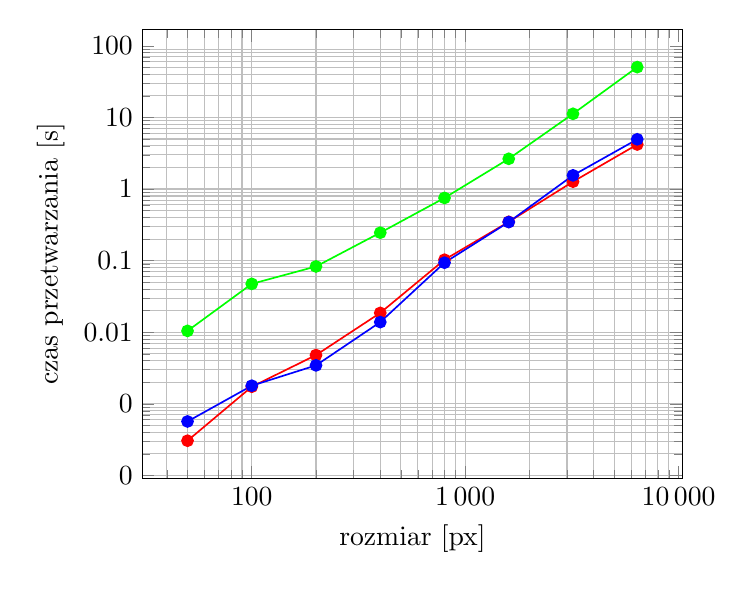
\begin{tikzpicture}
        \pgfplotsset{%
            x tick label style={/pgf/number format/1000 sep=\,},
            log base 10 number format code/.code={%
                $\pgfmathparse{10^(#1)}\pgfmathprintnumber{\pgfmathresult}$%
            }%
        }  
        \begin{axis}[
            grid=minor,
            xmode=log,
            ymode=log,
            xlabel={rozmiar [px]},
            ylabel={czas przetwarzania [s]},
            % xtick={50, 100, 200, 400, 800, 1600, 3200, 6400},
            log ticks with fixed point
        ]
            \addplot[mark=*, red, semithick] table {
                50 0.000305484
                100 0.00173367
                200 0.00479529
                400 0.0186251
                800 0.102972
                1600 0.348162
                3200 1.26685
                6400 4.18572
            };
            \addplot[mark=*, blue, semithick] table {
                50 0.00056756
                100 0.00179102
                200 0.00344637
                400 0.0138544
                800 0.0935612
                1600 0.345652
                3200 1.55231
                6400 4.94573
            };
            \addplot[mark=*, green, semithick] table {
                50 0.0104428 
                100 0.0473796 
                200 0.0828924 
                400 0.245594 
                800 0.750946 
                1600 2.64254 
                3200 11.2324 
                6400 50.3934 
            };
        \end{axis}
    \end{tikzpicture}
    \caption{Porównanie czasu zmiany obrazka 200x200px do docelowego rozmiaru w~zależności od długości boku kwadratowego obrazk}
    \label{fig:resizing-time}
\end{figure}

Zgodnie z~oczekiwaniami, najlepsze rezultaty zostały osiągnięte przez algorytm interpolacji dwukubicznej. Nawet przy dziesięciokrotnym powiększeniu, obrazek nadal wyglądał naturalnie i~zdecydowanie lepiej od pozostałych.  

Na wykresie~\ref{fig:resizing-time} przedstawiono zależność czasu przetwarzania od rozmiaru obrazka. Algorytmy najbliższego sąsiada oraz interpolacji dwuliniowej działają w~porównywalnym czasie, natomiast algorytm dwukubiczny znacznie odstaje od pozostałych dwóch, działając średnio o~rząd wielkości dłużej.

Na podstawie wykonanego eksperymentu, zdecydowałem się na wybór algorytmu interpolacji dwukubicznej. Krótki czas przetwarzania nie jest szczególnie oczekiwaną cechą od projektowanego systemu oraz algorytm będzie stosowany do zmniejszania obrazków a~nie do ich znacznego powiększania, dlatego też z~wszystkich trzech przedstawionych rozwiązań, algorytm dwukubiczny jest najlepszy.

\subsection{Filtracja zakłóceń}
\todo{Opisać algorytm filtracji zakłóceń - filtracja medianowa. Znaleźć źródła.}